\documentclass[a4j,12pt]{jreport}
\usepackage[dvipdfmx]{color}
\usepackage{color}
%\usepackage[dvips]{graphicx}
%\usepackage{multicol}
\usepackage{amsmath, ascmac, amssymb}
\usepackage{borderhead}
\usepackage[dvipdfmx]{graphicx}
\usepackage{graphicx}
\usepackage{subfigure}
\usepackage{multicol}
\usepackage{color}
\usepackage[dvipdfmx,breaklinks=true,a4paper=true,colorlinks,
linkcolor=black,citecolor=black,urlcolor=black]{hyperref}
\usepackage[dvipdfmx]{pxjahyper}
\usepackage{here}
\newcommand{\figref}[1]{\textgt{図 \ref{#1}}}
\newcommand{\tableref}[1]{\textgt{表 \ref{#1}}}
\newcommand{\chapterref}[1]{\textgt{第 \ref{#1} 章}}

\newcommand{\parfrac}[2]{\frac{\partial #1}{\partial #2}}
%\documentclass[a4j,12pt]{jarticle}
%%%%%行間の幅を再定義
\renewcommand{\baselinestretch}{1.15}
\renewcommand{\bibname}{参考文献}
%%%%%sectionで番号をつける深さ
%\setcounter{secnumdepth}{2}
%%%%%目次に書き出す深さ
\setcounter{tocdepth}{3}
\setcounter{secnumdepth}{3}
\setlength{\footskip}{7mm}
%%%%%%%%%%表紙
\begin{titlepage}
\vspace{-8cm}

\title{
	平成30年度 修士研究論文\vspace{1cm}\\
	\huge  レスキュー犬の一人称動画\\を用いた動作分類\vspace{6cm}
}

\author{
	電気通信大学大学院 情報理工学研究科\\
	情報学専攻 メディア情報学プログラム\\
	1730010\hspace{1cm}荒木 勇人\\
	主任指導教員 柳井 啓司 教授\\
        指導教員 橋本 直己 准教授
}

\date{
平成31年1月28日
}
\end{titlepage}



%%%%%%%%%%%%%%%%%%%%本文
\begin{document}

%%%%%%%%%%表紙
\maketitle
\thispagestyle{empty}
\pagebreak

\begin{abstract}

被災地での災害救助を補助する犬をレスキュー(災害救助)犬といい,カメラなどの計測装置を装備したレスキュー犬をサイバーレスキュー犬と言う.本研究では,犬にとりつけたセンサからサイバーレスキュー犬の活動を識別した.
光学センサと音声センサから得られた映像および音声データを含む動画像とCNNを用いて動作毎に分類するsound/image-based three-stream CNNの提案と,提案手法をマルチクラス推定に用いた実験を行なった.
光学センサから得られた情報は犬の一人称視点の映像である.これは通常,分類の対象とされる三人称視点の映像とは大きく異なる.
第三者視点映像は基本的に背景が動かず,前景となる被写体の動きを捉える.対して一人称視点映像は,センサそのものが動き回り,背景や前景が存在しない.
被写体の識別が主なアプローチとなる第三者視点映像の認識よりも,一人称視点映像の認識の難易度は非常に高いと言える.
sound/image-based three-stream CNNは動画から得られた静止画像・optical flow画像・音声を入力とする動画識別ネットワークである.
本提案手法の精度を示すため,3つの入力それぞれ単体とその組み合わせパターン
(静止画像単体,optical flow画像単体,音声単体,静止画像+optical flow画像,静止画像+音声,optical flow画像+音声)
を用いた識別との比較実験を行なった.
結果は,51.8\%で提案手法で最も高い精度が得られた.
推定には,レスキュー犬の訓練の様子を撮影したデータセットを用いた.このデータセットは現在も作成中であり,まだデータが十分とは言えない.
一人称視点動画からのマルチクラス推定というタスクと,レスキュー犬訓練データセットの複雑さのあいまったチャレンジングなタスクであることを踏まえると,本研究では次に繋がる十分な結果が得られたと言える.


\par


\end{abstract}

%%%%%%%%%%目次
%\pagestyle{plain}
\pagestyle{jgraduate}

\pagenumbering{roman}

\tableofcontents

\pagebreak

\pagenumbering{arabic}
\newpage

%%%%%%%%%%%%%%%%%%%%%%%%%%%%%%%%%%%%%%%%%%%%%%%%%%%%
%%%%%%%%%% 1章
\section{はじめに}
被災地での救助活動を行う際に,人間の補助として訓練されたレスキュー犬(災害救助犬)が探査を行う場合がある.レスキュー犬は,犬としての特性を生かして人間と協力して被災地の探索を行う.がれきの隙間などの狭い空間,倒壊した建物など人間には踏破困難な環境でも探査可能であり,また発達した嗅覚を頼りにした救助活動が可能である.しかし,彼らは人間に向けた言語を持たないため,人間はレスキュー犬の行動から彼らが収集した情報を理解しなくてはならない.現状では,レスキュー犬を指揮するハンドラーと呼ばれる人間がレスキュー犬の行動を手動でマーキングしており,その情報を消防などの指揮命令者に口頭伝達している.このレスキュー犬との共同探索の問題点として,トリアージ(緊急度に従った手当の優先順位付け)のための周辺環境情報や,要救助者情報の不足があげられる.また,ハンドラーによる記録はどうしても主観的になり客観性が不足し,さらにそれを口頭伝達することで正確性がより不足する.

本研究では,レスキュー犬にセンサを装着して得られたデータ用いてレスキュー犬の行動をリアルタイムに分類すること目的とする.深層学習を用いた画像識別にある既存手法を予備実験として行った.予備実験をもとに,動画からのレスキュー犬行動分類を行う.本研究は映像だけでなく音声などのデータも活用したマルチモーダルな動画分類である.本研究により,レスキュー犬が今何をしているのか明示的に判断することが可能となり,トリアージに必要な情報が整理され,災害救助活動の効率化が期待される.

\section{関連研究}

レスキュー犬の行動をモニタリングするために,濱田,大野らによって装着型計測・記録装置が開発された~\cite{dog01}.図\ref{cyber}にレスキュー犬に装着可能な軽量な行動計測スーツ示す.これを着用したレスキュー犬はサイバー救助犬とも呼ばれる.各種センサを用いた計測データを記録し,リアルタイムに映像などのデータを無線配信することが可能である.そのため,レスキュー犬が人の目の及ばない範囲で活動する際にもレスキュー犬の行動やその周辺環境などを把握するのに役立つ.サイバー救助犬は,政府による総合科学技術・イノベーション会議が研究開発を促進しているImPACTというプログラムのタフ・ロボティクス・チャレンジの一環である.
タフ・ロボティクス・チャレンジとは災害救助を目的としたロボットの研究開発プロジェクトであり,その中で,災害救助用サイボーグ犬の開発の足掛かりとしてサイバー救助犬が研究されている.

\begin{figure}[htbp]
 \begin{center}
  \includegraphics[width=6cm]{./Img/cyberdog.eps}
  \caption{装着型計測・記録装置~\cite{dog01}より引用}
  \label{cyber}
 \end{center}
\end{figure}

また,Ehsanらによる犬の一人称視点動画からの犬行動予測の研究がある~\cite{whoretthedog}.これは,犬の行動をモデリングし,犬が次にどのような道をたどり行動するかを予測している.

%\section{問題点}
しかし,これらの研究は犬の行動のモデリングであり,犬の周辺環境の推定などは行っていない.また,入力は動画像のみであり,音声などのデータは利用していない.レスキュー犬の課題には,犬の周辺環境情報や動画像からだけでは判断できない情報の取得が含まれている.例えばレスキュー犬は要救助者を発見するとその場で待機し吠え続けるように訓練されている.このように,動画像データからだけではなく,音声データ,および慣性データ・GPSデータなどの情報を複合的に用いてレスキュー犬の状態を判断しなければならない.本研究は動画像と音声からなるマルチモーダルな情報を入力とした犬の行動の分類を目的としている. 

\section{手法概要}
動画からレスキュー犬の行動を推定するための手法の概要は以下の通りである.
\begin{itemize}
 \item 動画から一定フレームと対応する音声を取出し整形.
 \item LSTMなどの時系列情報を扱う手法により,データから特徴量を抽出.
 \item 単位データから犬行動を分類するよう学習し,分類.
\end{itemize}

\section{予備実験}
データセットに犬の一人称視点動画DogCentric Activity Dataset(DCAD)~\cite{yumi2014first}を用い,これを分類する予備実験を行った.これは犬の散歩を記録したデータであり,災害救助活動やその訓練データではない.災害救助活動および訓練データは現在作成中である.
DCADデータセットは10クラス209クリップで構成されている.クラスはそれぞれ,横断前の待機\(Car\), 水分の摂取\(Drink\), 手渡しでの食事\(Feed\), 左を見る\(Look\_at\_Left\), 右を見る\(Look\_at\_Right\), 人間が犬を撫でる\(Pet\),ボールで遊ぶ\(Play\_with\_ball\), 体をブルブルと振る\(Shake\), 何かの臭いを嗅ぐ\(Sniff\), 歩く\(Walk\),である.

\begin{figure}[htbp]
%  \begin{center}
    \begin{tabular}{c}
     % 0
      \begin{minipage}{0.18\hsize}
        \begin{center}
          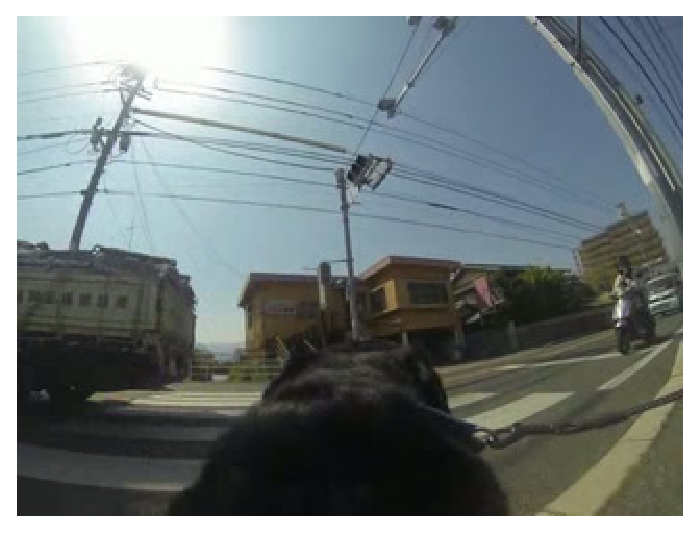
\includegraphics[clip, width=1.7cm]{./Img/HC005.eps}
          \hspace{0.3cm} { }
        \end{center}
      \end{minipage}
      \begin{minipage}{0.18\hsize}
        \begin{center}
          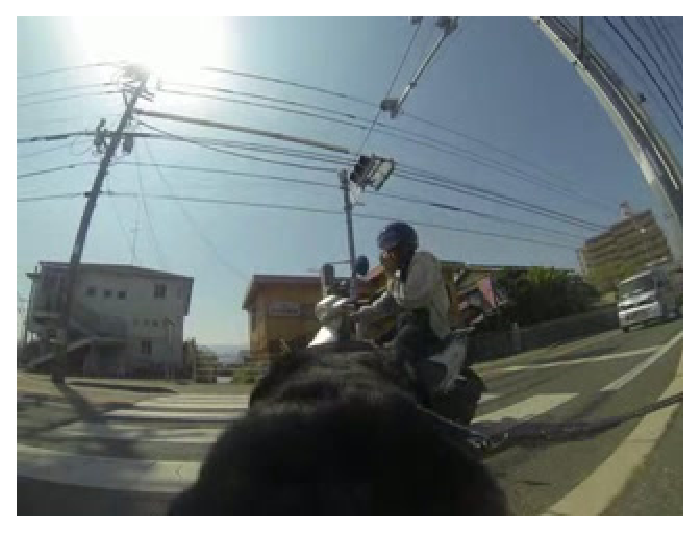
\includegraphics[clip, width=1.7cm]{./Img/HC006.eps}
          \hspace{0.3cm} { }
        \end{center}
      \end{minipage}

      % 2
      \begin{minipage}{0.18\hsize}
        \begin{center}
          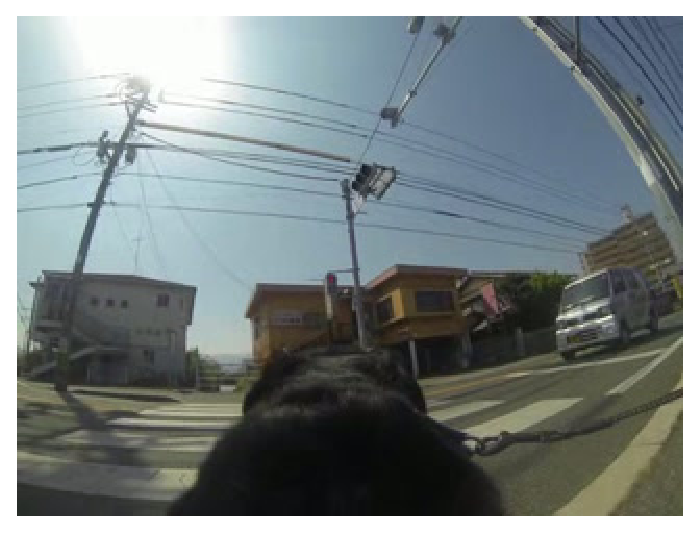
\includegraphics[clip, width=1.7cm]{./Img/HC007.eps}
          \hspace{0.0cm} {Car}
        \end{center}
      \end{minipage}

      % 4
      \begin{minipage}{0.18\hsize}
        \begin{center}
          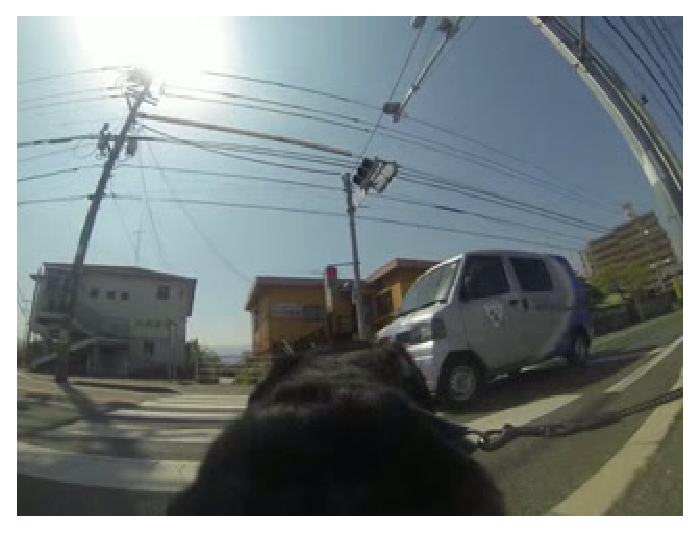
\includegraphics[clip, width=1.7cm]{./Img/HC008.eps}
          \hspace{0.1cm} { }
        \end{center}
      \end{minipage}
      % 5
      \begin{minipage}{0.18\hsize}
        \begin{center}
          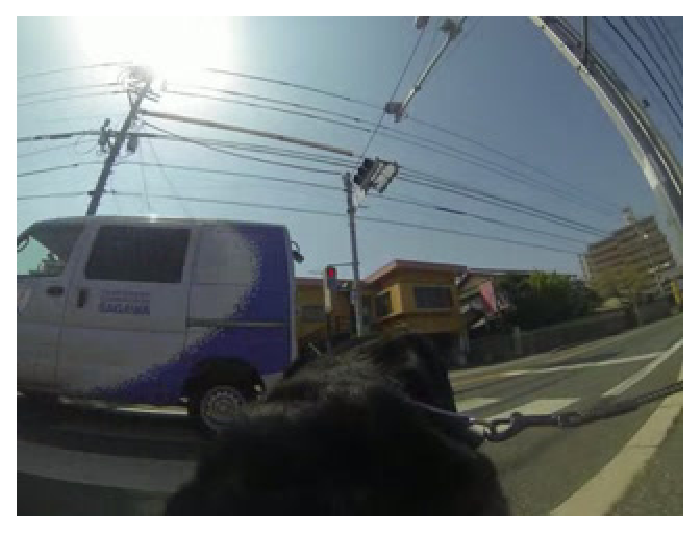
\includegraphics[clip, width=1.7cm]{./Img/HC009.eps}
          \hspace{0.2cm} { }
        \end{center}
      \end{minipage}
\\
     \begin{minipage}{0.18\hsize}
      \begin{center}
       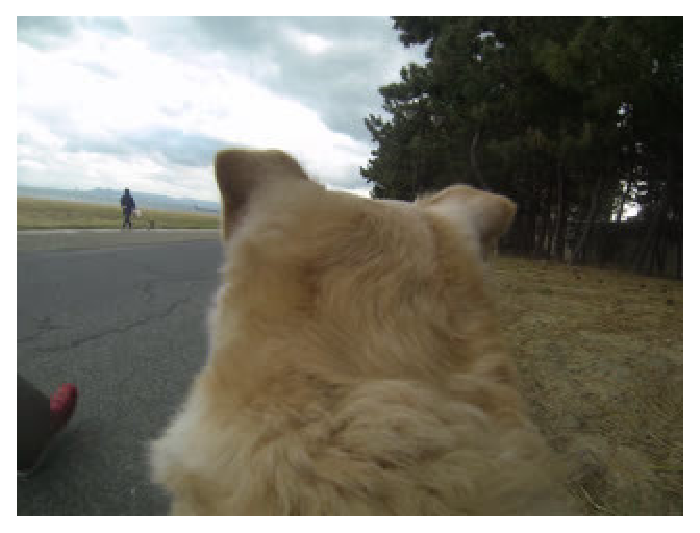
\includegraphics[clip, width=1.7cm]{./Img/KL001.eps}
       \hspace{0.3cm} { }
      \end{center}
     \end{minipage}
     \begin{minipage}{0.18\hsize}
      \begin{center}
       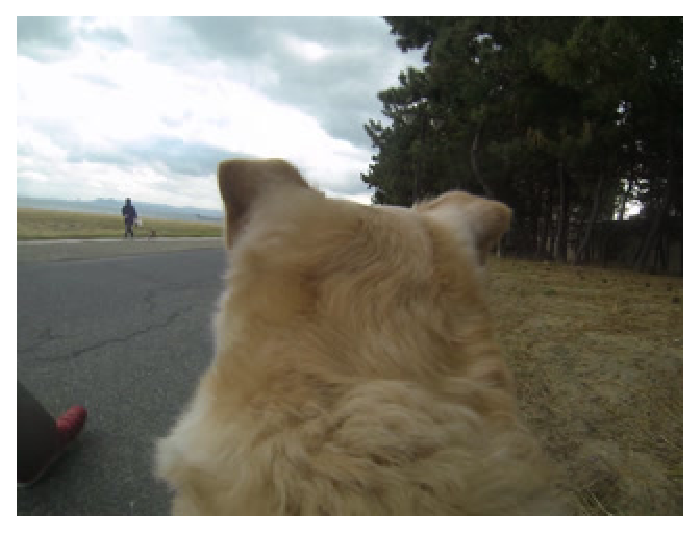
\includegraphics[clip, width=1.7cm]{./Img/KL002.eps}
       \hspace{0.3cm} { }
      \end{center}
     \end{minipage}
     \begin{minipage}{0.18\hsize}
      \begin{center}
       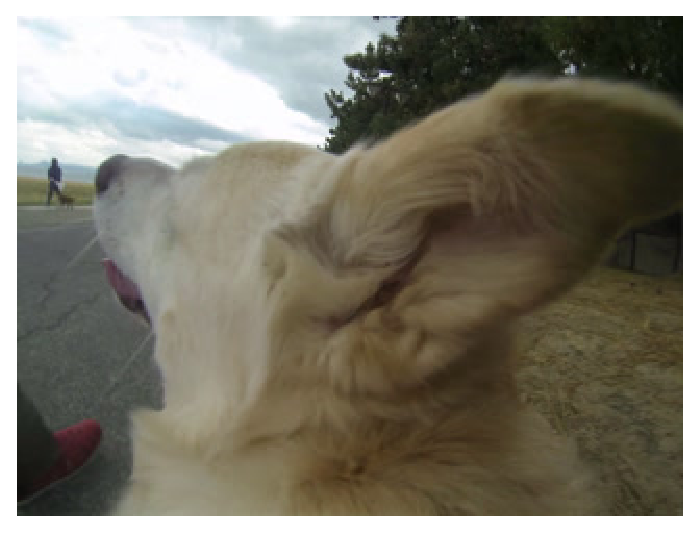
\includegraphics[clip, width=1.7cm]{./Img/KL003.eps}
       \hspace{0.1cm} {Look\_at\_Left} 
      \end{center}
     \end{minipage}
     \begin{minipage}{0.18\hsize}
      \begin{center}
       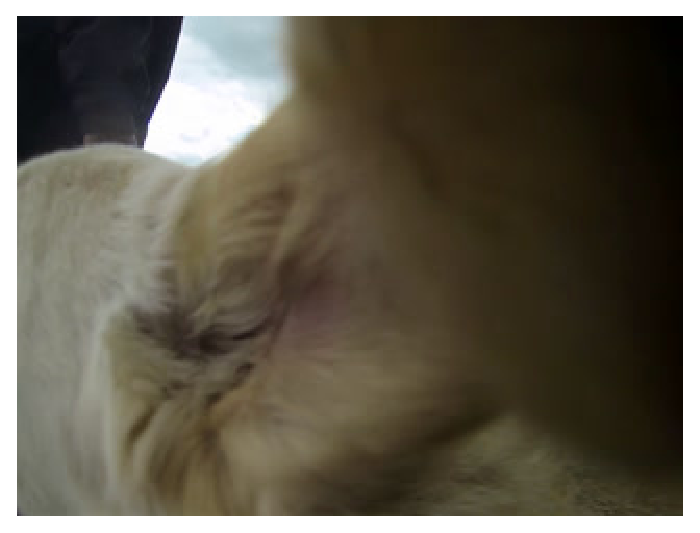
\includegraphics[clip, width=1.7cm]{./Img/KL004.eps}
       \hspace{1.3cm} { } 
      \end{center}
     \end{minipage}
     \begin{minipage}{0.18\hsize}
      \begin{center}
       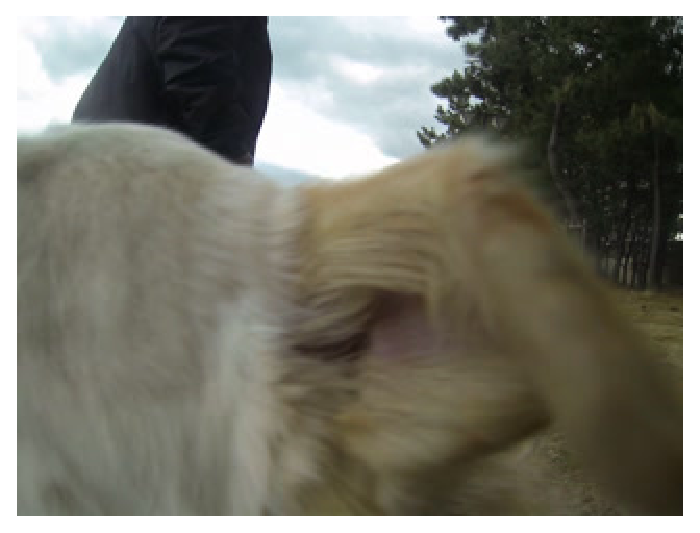
\includegraphics[clip, width=1.7cm]{./Img/KL005.eps}
       \hspace{1.6cm} { }
      \end{center}
     \end{minipage}

    \end{tabular}
    \caption{DogCentric Activity Dataset}
    \label{dcad_img}
%  \end{center}
\end{figure}

動画ひとつにつきフレーム全体の平均を取り~(式\ref{frame}\}),画像として扱い分類した~(図\ref{net}).ResNetとVGG16をそれぞれ用いたPre-trained modelのfine-tuningと二通り行った.

\begin{equation}
 \label{frame}
 Input = \frac{\Sigma^{sec \times FPS} Frame}{sec \times FPS}
\end{equation}

\begin{figure}[htbp]
 \begin{center}
  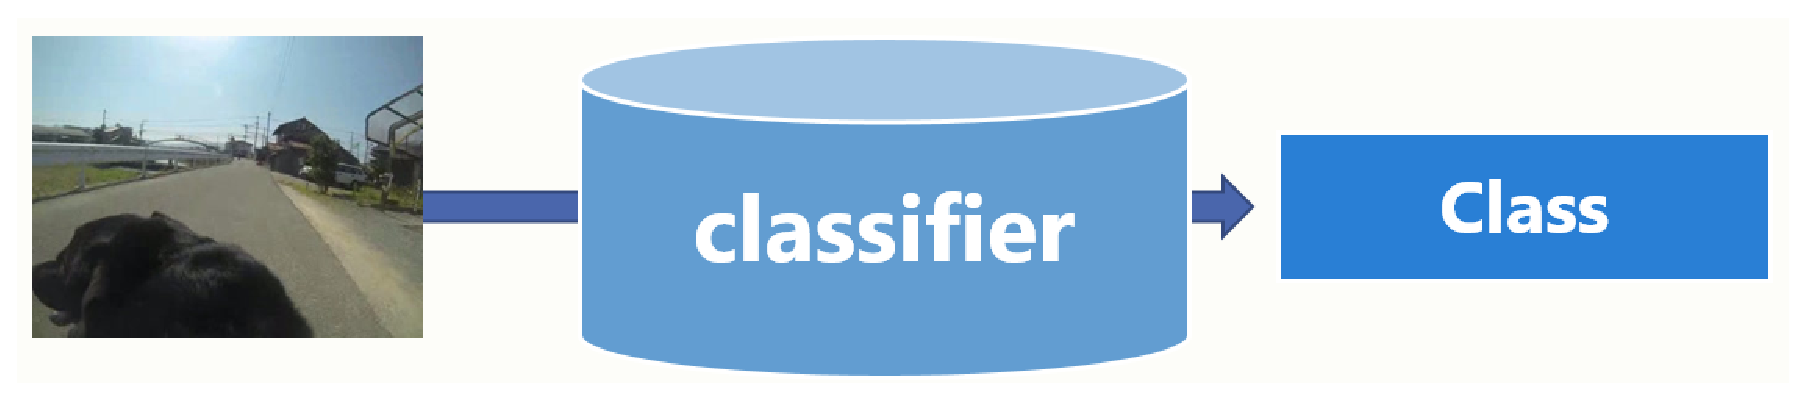
\includegraphics[width=8cm]{./Img/net.eps}
  \caption{ネットワーク}
  \label{net}
 \end{center}
\end{figure}

% \begin{figure}[htbp]
%  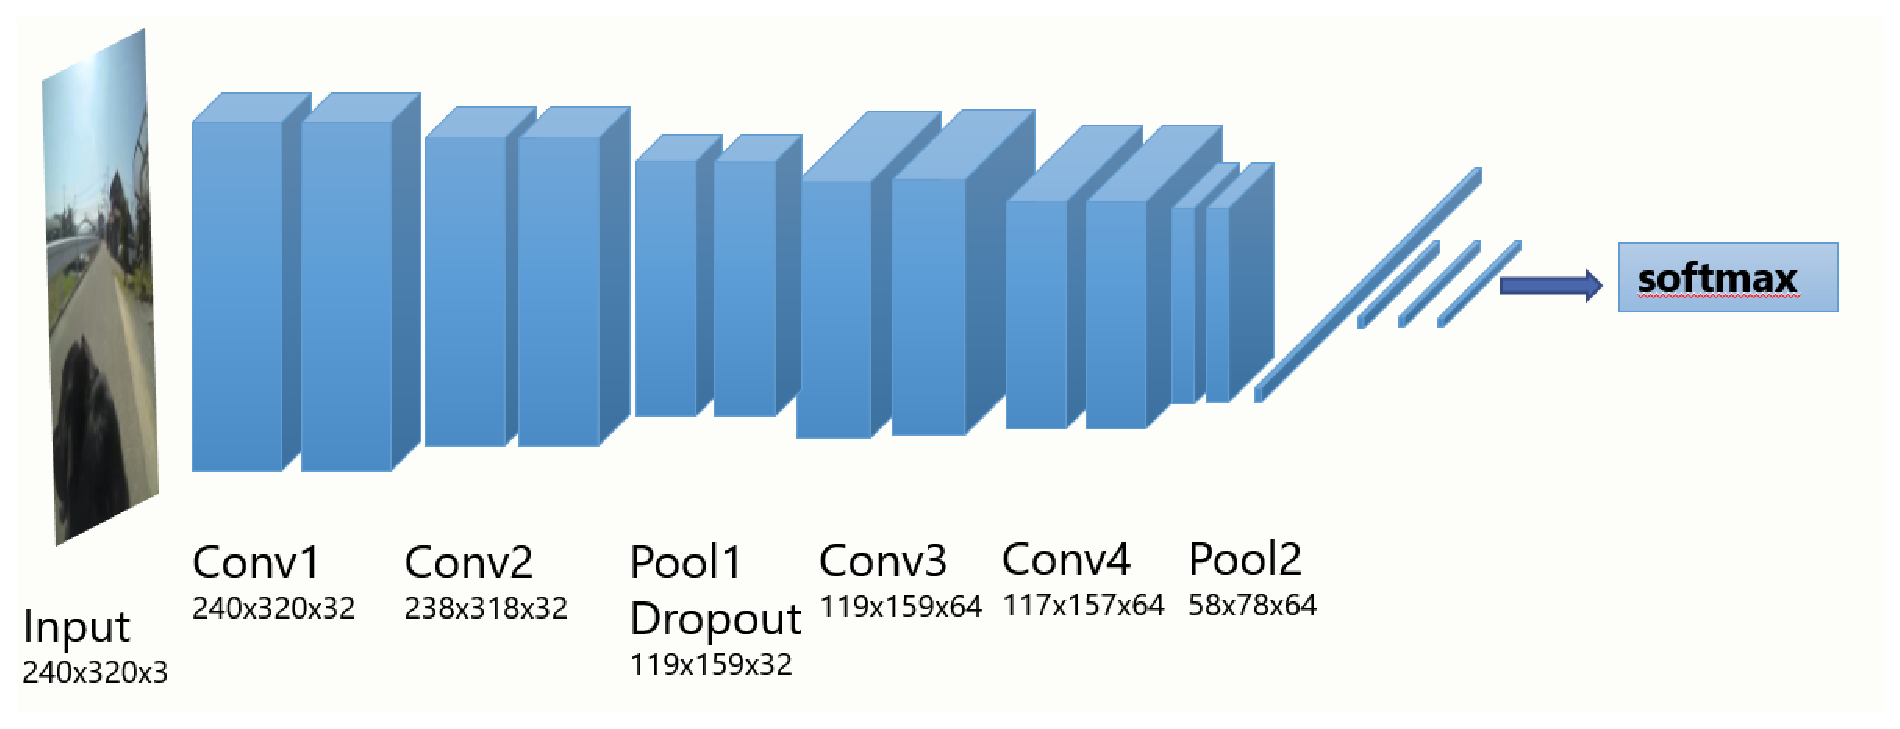
\includegraphics[width=10cm]{./Img/usemodel.eps}
%  \caption{利用したモデル}
%  \label{model}
% \end{figure}
% \begin{figure}[htbp]
%  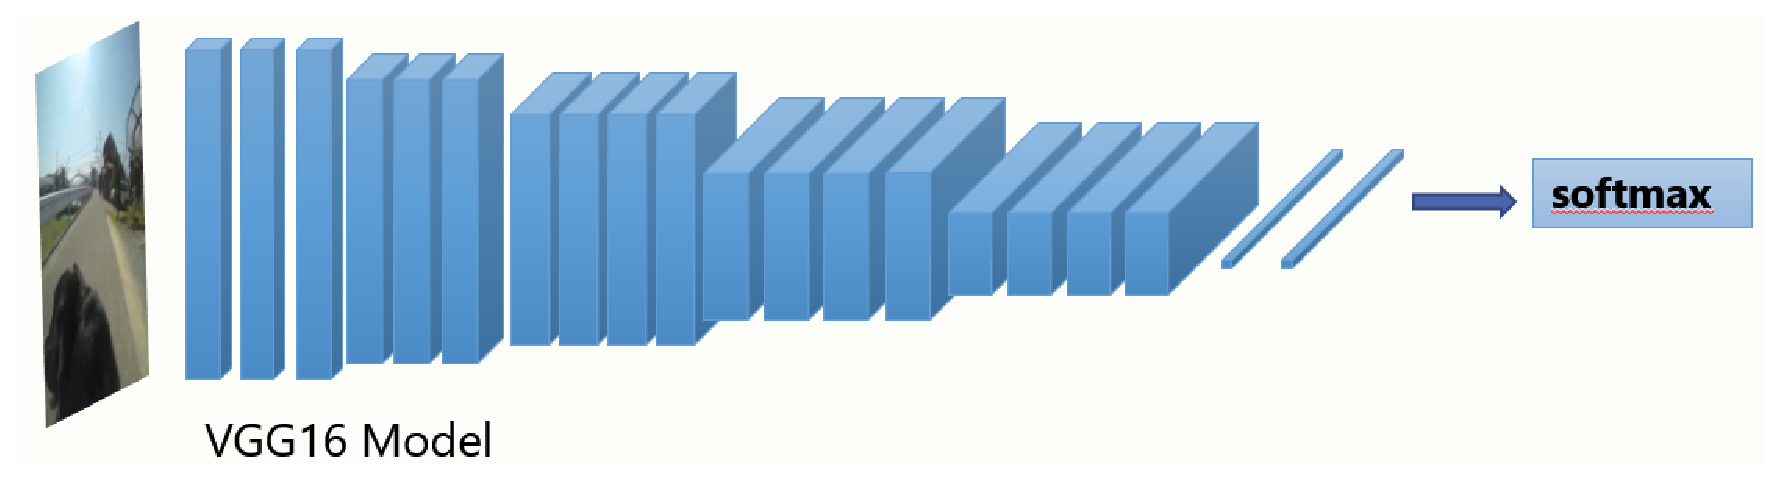
\includegraphics[width=8cm]{./Img/vgg16model.eps}
%  \caption{VGG16モデル}
%  \label{vgg16model}
% \end{figure}
\section{実験結果}
予備実験の結果を~(図\ref{vgg16_res},\ref{resnet_res})にそれぞれ示す.分類率は,VGG16モデルを利用したものが64.3\%,ResNetモデルを利用したものが59.5\%であった.
全般的に,データの多いクラスは精度が高い傾向にあるが,データの少ないクラスは精度が低い傾向にある.
加えて,~\(Car\)クラスは道路の進行方向に対して垂直に待機している10クラスの中で特殊なクラスであり,車などの写ったフレームの影響で分類精度が上昇していると考えられる.~\(Feed\)クラス,~\(Pet\)クラス,~\(Play\_with\_ball\)クラスは,それぞれフレーム内を人間が占める割合が多いクラスと言え,そのため混同が起こりやすいと考えられる.

%\(Look_at_Left\)クラスは


\begin{figure}[htbp]
 % \begin{tabular}{cc}
 %  \begin{minipage}{0.5\textwidth}
   \begin{center}
    
    \includegraphics[scale=0.3]{./Img/vgg16_res.eps}
    \caption{VGG16 pretrained modelによるfinetuningの結果}
    \label{vgg16_res}
   \end{center}
  % \end{minipage}
  % \begin{minipage}{0.5\textwidth}
\end{figure}
\begin{figure}[htbp]

   \begin{center}

    \includegraphics[scale=0.3]{./Img/resnet_res.eps}
  \caption{ResNet pretrained modelによるfinetuningの結果}
  \label{resnet_res}
   \end{center}
 %  \end{minipage}
 % \end{tabular}

\end{figure}

\section{まとめ,今後の課題}
動画の各フレームの平均を取り,画像として識別した.
データの少ないクラスは精度が低いため,データを補う必要がある.
予備実験では簡易的な方法を用いたが,今後は最新手法による分類を検討している.またレスキュー犬の行動を認識する際には複数クラスの出力にする必要がある.


今後の課題として,時系列情報を特徴量抽出に使う.
また,音声データから特徴量を抽出し,動画特徴量と併せたマルチモーダルな特徴量を利用し,レスキュー犬の行動分類を行う.


{\scriptsize % 7pt
%{\footnotesize % 8pt
%{\small % 9pt
%\bibliographystyle{ieee}
\bibliographystyle{junsrt}
\bibliography{ref}
}
% \begin{footnotesize}
% %{\small
% \bibliography{ref}
% \bibliographystyle{junsrt}
% %}
% \end{footnotesize}
\end{document}

%%%%%%%%%%%%%%%%%%%%%%%%%%%%%%%%%%%%%%%%%%%%%%%%%%%%
%%%%%%%%%% 2章
\chapter{関連研究}
本研究では犬の一人称視点動画からの犬の活動分類を行う.人間のライフログとしての一人称動画の分類や,車載映像からの車の行動推定,第三者視点での動画分類,音声を用いた動画分類などについて紹介し,本研究との関連を述べる.
\section{画像認識}
\section{動画認識}
\subsection{Optical flow}
\subsubsection{FlowNet2.0}
\subsection{Two-stream}
\subsection{3D Convolution}
\section{音声分類}
\subsection{Sound Net}
\subsection{Audio-Visual Scene Analysis}

%%%%%%%%%% 3章
\chapter{提案手法}
本研究では犬の行動推定のために,動画像・音声のマルチラベル分類を行った.
まず,入力となる動画から静止画像のフレーム($F_t$)を取り出し,直後の$F_{t+1}$間とのoptical flow画像($O_t$)を生成する.次に両画像から同じ構造の2つのネットワークを用いて特徴量の抽出を行う.
そして対応する音声($A_t$)からメル周波数ケプストラム係数($M_t$)を求め,前述とは異なる構造のネットワークを用いて($M_t$)から特徴量の抽出を行う.
最後にこれら2つあるいは3つの特徴量の組み合わせ毎に結合し,分類ネットワークでクラス分類を行う.
この際に,音声をフレームと同じサイズで切り出すと特徴が著しく失われるため入力音声には$F_t$の前後0.5秒ずつを用いた.動画あるいは音声から実際に犬の行動を推定する場合を想定し,現実的で取り扱いやすい時間としてこれを設定した.

分類はフレーム毎に行った.
\section{音声と画像を用いたSound based Two-stream network}
1つ目の提案手法として,音声を用いたTwo-stream networkを提案する.
既存のTwo-stream networkを改造し,静止画と音声からの動画分類の手法である.
Two-stream networkと違い音声を用いるため,これをSound based Two-stream networkと呼称する.
Sound based Two-stream networkのアーキテクチャを図~\ref{sound-two-stream}に示す.
本研究ではこのネットワークをクラス分類ではなくマルチクラス推定に用いる.
%音声と静止画を用いたマルチクラス分類
%音声とoptical flow画像を用いたマルチクラス分類

\begin{figure}[htbp]
 \begin{center}
  \includegraphics[width=15cm]{./Figures/soundbasedTwostream.eps}
  \caption{Sound based Two-stream (提案手法)のアーキテクチャ.(3,224,224)次元の画像と(1,20,94)次元を音声をそれぞれ別のネットワークに通し,得られた特徴を結合したのちFCレイヤを通しクラス数と同じ次元の出力を得る.}
  \label{sound-two-stream}
 \end{center}
\end{figure}



\section{音声・静止画像・optical flow画像を用いたSound based Three-stream network}
2つ目の提案手法として,音声,静止画像,optical flow画像の3つの情報を用いたSound based Three-streamを提案する.
Sound based Two-stream networkに,画像を入力とするネットワークを加えた3つのstreamを組み合わせている.
Sound based Two-stream networkのアーキテクチャを図~\ref{sound-two-stream}に示す.


\begin{figure}[htbp]
 \begin{center}
  \includegraphics[width=15cm]{./Figures/soundbasedThreestream.eps}
  \caption{Sound based Three-stream (提案手法)のアーキテクチャ.(3,224,224)次元の画像と(1,20,94)次元を音声をそれぞれ別のネットワークに通し,得られた特徴を結合したのちFCレイヤを通しクラス数と同じ次元の出力を得る.}
  \label{sound-three-stream}
 \end{center}
\end{figure}

%%%%%%%%%% 4章
\chapter{提案手法}
本研究ではレスキュー犬行動推定のために,動画像・音声のマルチラベル分類を行う.
そのため,レスキュー犬訓練データセットを認識するための手法を提案する.

入力を動画とした際に,動画から静止画像と音声を切り出し,optical flow画像を生成する.
この3つをそれぞれ別のストリームに入力し,それぞれの出力を元にレスキュー犬の行動を推定する.概念図を~\ref{easy_image}に示す.
\begin{figure}[H]
 \begin{center}
  \includegraphics[width=10cm]{./Figures/easy_image.eps}
  \caption{提案手法の概要.入力動画から複数データを抽出し,それぞれ別のストリームへ入力する.各ストリームの出力をもとに,動画のレスキュー犬行動推定結果を最終出力とする.}
  \label{easy_image}
 \end{center}
\end{figure}

\section{音声と画像を用いたsound/image-based two-stream CNN}
1つ目の提案手法として,音声を用いたtwo-stream networkを提案する.
既存のtwo-stream networkを改造し,静止画と音声からの動画分類の手法である.
Two-stream networkと違い音声を用いるため,これをsound/image-based two-stream networkと呼称する.
sound/image-based two-stream networkのアーキテクチャを図~\ref{sound-two-stream}に示す.
これは画像ストリームと音声ストリームからなり,音声ストリームには音声から抽出したmfcc特徴を入力する.
画像ストリームには(3, 224, 224)次元の画像を入力とする.それぞれのストリームの出力を結合し,全結合層を通して各クラス毎の推定結果を得る.

本研究ではこのネットワークを一般的なシングルクラス分類ではなくマルチクラス推定に用いる.
まず入力となる動画から静止画像のフレーム($F_t$)を取り出し,直後の$F_{t+1}$間とのoptical flow画像($O_t$)を生成する.次に両画像から同じ構造の2つのネットワークを用いて特徴量の抽出を行う.
そして対応する音声($A_t$)からメル周波数ケプストラム係数($M_t$)を求め,前述とは異なる構造のネットワークを用いて($M_t$)から特徴量の抽出を行う.
最後にこれら2つあるいは3つの特徴量の組み合わせ毎に結合し,分類ネットワークでクラス分類を行う.
この際に,音声をフレームと同じサイズで切り出すと特徴が著しく失われるため入力音声には$F_t$の前後0.5秒ずつを用いた.動画あるいは音声から実際に犬の行動を推定する場合を想定し,現実的で取り扱いやすい時間としてこれを設定した.
分類はフレーム毎に行った.

シングルクラス分類の損失関数にはCrossEntropyLossを用いてクラス確率を求めたが,マルチクラス推定にはクラス毎にSoftMarginLossを用いた.
入力を$x$,出力を$y$,クラス数を$C$とすると,マルチクラス推定の損失関数SoftMarginLossは式~\ref{softmargin}に定義される.
推定クラスが正解なら$\Sigma$内の第2項,不正解なら第1項が計算に利用するように設計されており,推定ラベルによって関数が変わる.
本研究では11クラスあり,出力yは11次元のバイナリとする.
閾値=0.5とし,閾値以上のクラスを推定クラスとした.
\begin{equation}
\label{softmargin}
loss(x, y) = -\frac{1}{C} * \Sigma_{i} y[i] * log((1+exp(-x[i]))^{-1}) + (1 - y[i]) * log(\frac{exp(-x[i])}{1+exp(-x[i])})
\end{equation}

学習は全てにおいて100エポック行った.学習率は1e-03〜1e-06,バッチサイズは32〜128の範囲で学習毎に変え制限の中で最も良い精度の結果を評価した.


\begin{figure}[htbp]
 \begin{center}
  \includegraphics[width=15cm]{./Figures/soundbasedTwostream.eps}
  \caption{Sound/image-based two-stream CNN(提案手法)のアーキテクチャ.(3,224,224)次元の画像と(1,20,94)次元を音声をそれぞれ別のネットワークに通し,得られた特徴を結合したのちFCレイヤを通しクラス数と同じ次元の出力を得る.}
  \label{sound-two-stream}
 \end{center}
\end{figure}



\section{音声・静止画像・optical flow画像を用いたsound/image-based three-stream CNN}
2つ目の提案手法として,音声,静止画像,optical flow画像の3つの情報を用いたsound/image-based three-streamを提案する.
Sound/image-based two-stream networkに,画像を入力とするネットワークを加えた3つのstreamを組み合わせている.
Sound/image-based two-stream networkのアーキテクチャを図~\ref{sound-two-stream}に示す.
動画を31フレームとし,中央から切り出した静止画像とそれに対応する直後のoptical flow画像をそれぞれImageNetで学習済みのVGG16モデルに通し,畳み込み層の出力を結合する.
動画から切り出した音声は音声ストリームに入力する.畳み込みを繰り返すと特徴の縦横次元が小さくなるため,静止画像の畳み込みの出力と同じサイズになるように調整する.
調整は畳み込みで奥行き次元を揃えた後,同じ特徴をリピートし目的の大きさになるまでコピーして結合する.
本研究では入力音声は(1,20,94)次元の特徴に変換しており,畳み込みを繰り返して(512,1,1)次元にする.この細長い特徴を縦横に7つ並べ,(512,7,7)の特徴として静止画像とoptical flowの結合特徴に追加で結合する.

\begin{figure}[htbp]
 \begin{center}
  \includegraphics[width=15cm]{./Figures/soundbasedThreestream.eps}
  \caption{Sound/image-based three-stream CNN(提案手法)のアーキテクチャ.(3,224,224)次元の画像と(1,20,94)次元を音声をそれぞれ別のネットワークに通し,得られた特徴を結合したのちFCレイヤを通しクラス数と同じ次元の出力を得る.}
  \label{sound-three-stream}
 \end{center}
\end{figure}

%%%%%%%%%% 5章
\chapter{実験}
本章では予備実験2種類を含む全9種類の実験について説明を行う.
予備実験として,DCADとレスキュー犬訓練データセットをクリップセットとしてまとめたもののクラス分類を行なった.
犬の一人称動画は人間の一人称動画とは大きく異なる.そのため,この予備実験では犬一人称動画分類タスクに対するCNNの有効性を確認した.

本実験では,Sound based Three-stream networkを用いてレスキュー犬訓練データセットのマルチクラス推定を行なった.
提案手法の有用性を示すためのアブレーションスタディに
静止画像からのマルチラベル推定,
optical flow画像からのマルチラベル推定,
音声データからのマルチラベル推定2種,
Sound based Two-stream networkを用いた音声データと静止画像からのマルチクラス推定,
同じくSound based Two-stream networkを用いた音声データとoptical flow画像からのマルチクラス推定
をそれぞれ行なった.
\section{DCAD}
DCADはクリップ毎にフレーム間の平均をとり,画像として扱ってVGG16のpretrained modelを用いてfinetuningを行なった.
予備実験の結果を図~\ref{vgg16_res}に示す.分類率は64.3\%であった.
Iwashitaらによる局所的特徴量を用いた分類実験での精度は60.5\%であった.このことから,犬一人称視点動画においてCNNの有効性が示された.

全般的に,データの多いクラスは精度が高い傾向にあるが,データの少ないクラスは精度が低い傾向にある.
加えて,~\(Car\)クラスは道路の進行方向に対して垂直に待機している10クラスの中で特殊なクラスであり,車などの写ったフレームの影響で分類精度が上昇していると考えられる.~\(Feed\)クラス,~\(Pet\)クラス,~\(Play\_with\_ball\)クラスは,それぞれフレーム内を人間が占める割合が多いクラスと言え,そのため混同が起こりやすいと考えられる.

\begin{figure}[H]
 % \begin{tabular}{cc}
 %  \begin{minipage}{0.5\textwidth}
   \begin{center}

    \includegraphics[scale=0.5]{./Figures/vgg16_res.eps}
    \caption{VGG16 pretrained modelとDCADによるfinetuningの結果}
    \label{vgg16_res}
   \end{center}
  % \end{minipage}
  % \begin{minipage}{0.5\textwidth}
\end{figure}

\section{レスキュー犬訓練シングルクラス分類}
レスキュー犬訓練データセットは動画をラベル毎に切り出して短いクリップ群を作り,そのクリップ毎に同様にフレーム間の平均を取った画像を作成しVGG16のpretrained modelを用いてfinetuningした.
\subsection{動画平均画像}
レスキュー犬訓練データセットでの予備実験の結果を図~\ref{sub_resque_res}に示す.

データ数の多いwalkクラスやstopクラスだけでなく,shakeクラスやeatクラスなどのデータ数の少ないクラスも大まかに分類できていることが分かる.
この結果によって,レスキュー犬訓練データセットからクラス分類・推定が可能であることが示された.
\begin{figure}[H]
  \begin{center}
    \includegraphics[scale=0.7]{./Figures/resque_mean_result.eps}
    \caption{VGG16 pretrained modelとレスキュー犬訓練データセットフレーム平均画像によるクラス分類のfinetuning結果}
    \label{sub_resque_res}
  \end{center}
\end{figure}

\subsection{オプティカルフロー動画平均画像}
動画像のフレーム間の平均を取った手法と同様に,クリップ毎にoptical flowの平均画像を作成しVGG16のpretrained modelを用いてfinetuningを行なった.
結果を図~\ref{sub_optresque_res}に示す.

やはりデータ数の影響を受けているものの,通常の動画のフレーム平均画像とは異なる傾向が得られた.
この結果によって,optical flow画像から得られる特徴の有用性が示された.
\begin{figure}[H]
  \begin{center}
    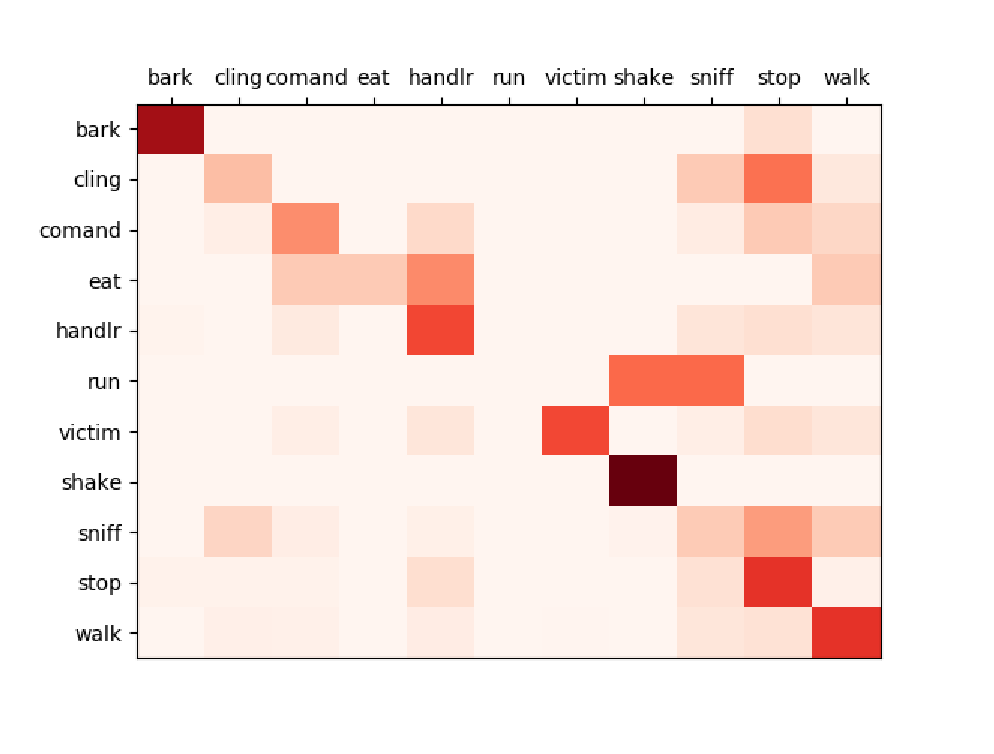
\includegraphics[scale=0.7]{./Figures/resque_optmean_result.eps}
    \caption{VGG16 pretrained modelとレスキュー犬訓練データセットoptical flow動画フレーム平均画像によるクラス分類のfinetuning結果}
    \label{sub_optresque_res}
  \end{center}
\end{figure}

%%%%%%%%%% 6章
\chapter{実験結果}
\section{予備実験}
予備実験の結果を~(図\ref{vgg16_res},\ref{resnet_res})にそれぞれ示す.分類率は,VGG16モデルを利用したものが64.3\%,ResNetモデルを利用したものが59.5\%であった.
全般的に,データの多いクラスは精度が高い傾向にあるが,データの少ないクラスは精度が低い傾向にある.
加えて,~\(Car\)クラスは道路の進行方向に対して垂直に待機している10クラスの中で特殊なクラスであり,車などの写ったフレームの影響で分類精度が上昇していると考えられる.~\(Feed\)クラス,~\(Pet\)クラス,~\(Play\_with\_ball\)クラスは,それぞれフレーム内を人間が占める割合が多いクラスと言え,そのため混同が起こりやすいと考えられる.

%\(Look_at_Left\)クラスは


\begin{figure}[htbp]
 % \begin{tabular}{cc}
 %  \begin{minipage}{0.5\textwidth}
   \begin{center}
    
    \includegraphics[scale=0.3]{./Figures/vgg16_res.eps}
    \caption{VGG16 pretrained modelによるfinetuningの結果}
    \label{vgg16_res}
   \end{center}
  % \end{minipage}
  % \begin{minipage}{0.5\textwidth}
\end{figure}
\begin{figure}[htbp]

   \begin{center}

    \includegraphics[scale=0.3]{./Figures/resnet_res.eps}
  \caption{ResNet pretrained modelによるfinetuningの結果}
  \label{resnet_res}
   \end{center}
 %  \end{minipage}
 % \end{tabular}
\end{figure}
\section{シングルクラス分類}
\subsection{動画像平均画像クラス認識}
\subsection{オプティカルフロー画像クラス認識}
\subsection{音声クラス認識}
\subsection{音声と動画のマルチモーダル情報クラス認識}


\section{マルチクラス認識}
\subsection{動画像平均画像クラス認識}
\subsection{オプティカルフロー画像クラス認識}
\subsection{音声クラス認識}
\subsection{音声と動画のマルチモーダル情報クラス認識}


%%%%%%%%%% 7章
%\section{考察}
全体の結果を表~\ref{expetiments_result}に示す.



\begin{table}[tb]
 \centering
 \caption{各実験比較表}\label{expetiments_result}
 \scalebox{0.80}[0.80]{
  \begin{tabular}{|l||c|c|c|c|c|c|c|c|c|c|c|c|}
   \hline \hline
   & \rotatebox{90}{bark}& \rotatebox{90}{cling}&\rotatebox{90}{command}& \rotatebox{90}{eat}&\rotatebox{90}{handler}& \rotatebox{90}{run}&\rotatebox{90}{victim}& \rotatebox{90}{shake}& \rotatebox{90}{sniff}& \rotatebox{90}{stop}& \rotatebox{90}{walk} & \rotatebox{90}{全体}\\ \hline
静止画像   & 0.244& 0.066& 0.0& 0.024& 0.057& 0.0& 0.204& 0.0& 0.0& 0.588& 0.51&  0.436 \\ \hline
optical flow   & 0.141& 0.0& 0.0& 0.0& 0.017& 0.0& 0.017& 0.0& 0.0& 0.586& 0.476&  0.406 \\ \hline
音声 (Conv1D)   & {\bf 0.669}& 0.078& 0.22& 0.023& 0.138& 0.0& 0.274& {\bf 0.44}& 0.502& 0.745& 0.704&  0.512 \\ \hline
音声 (Conv2D)   & 0.563& 0.04& 0.188& 0.001& 0.059& 0.0& 0.201& 0.304& 0.524& 0.744& 0.74&  0.512 \\ \hline
静止画像+optical   & 0.11& 0.018& 0.043& 0.0& 0.155& 0.0& 0.259& 0.0& 0.426& 0.705& 0.668&  0.435 \\ \hline
静止画像+音声   & 0.662& 0.031& 0.195& 0.018& 0.115& 0.002& 0.308& 0.402& 0.498& 0.726& 0.694&  0.5 \\ \hline
optical flow+音声   & 0.667& 0.054& {\bf 0.234}& 0.014& 0.123& 0.01& 0.223& 0.356& 0.487& 0.759& 0.692&  0.493 \\ \hline
静止+optical+音声   & 0.577& {\bf 0.135}& 0.186& {\bf 0.066}& {\bf 0.183}& {\bf 0.026}& {\bf 0.433}& 0.409& {\bf 0.53}& {\bf 0.779}& {\bf 0.725}& {\bf 0.518} \\ \hline
  \end{tabular}
 }
\end{table}




\chapter{まとめ,今後の課題}
Sound based Three-streamの提案と,提案手法を用いたレスキュー犬の行動推定を行なった.
提案手法との比較のために行なった実験は以下である.
\begin{itemize}
  \item 静止画像からの犬行動マルチラベル推定
  \item optical flow画像からの犬行動マルチラベル推定
  \item 音声からの犬行動マルチラベル推定
  \item 静止画像とoptical flow画像からの犬行動マルチラベル推定
  \item 音声と静止画像からの犬行動マルチラベル推定
  \item 音声とoptical flow画像からの犬行動マルチラベル推定
  \item 音声と静止画とoptical flow画像からの犬行動マルチラベル推定
\end{itemize}
結果は提案手法が最も高く,音声・静止画像・optical flow画像のそれぞれに必要な情報が含まれており,3つのデータにそれぞれ必要な情報が含まれているとわかった.
精度は51.2\%と数値では決して高いとは言えないが,約30fpsの動画で1/5フレーム毎に行なった推定の結果であるため非実用的とも言えない結果となった.

今回は研究の範囲としなかったが,レスキュー犬行動動画の入力に対してリアルタイムに結果を出すことも求められる.
また,実験に対する疑問として音声フレームの長さはどの程度か適しているのか判断できていない.
これの変更でどの程度影響があるのかを検証し,より適切な音声フレーム長が判断できればより高い精度も期待できる.

%{\scriptsize % 7pt
%{\footnotesize % 8pt
%{\small % 9pt
%\bibliographystyle{ieee}
\bibliographystyle{junsrt}
\bibliography{ref}
%}
% \begin{footnotesize}
% %{\small
% \bibliography{ref}
% \bibliographystyle{junsrt}
% %}
% \end{footnotesize}
\end{document}


%%%%%%%%%% 目次に参考文献を加える
\addcontentsline{toc}{chapter}{参考文献}
%%%%%%%%%% 参考文献
\bibliographystyle{junsrt}
\bibliography{bib}

%付録があればここで書く
%%%%%%%%%% 付録A
%%%%%%%%%% 付録B
%\input{}

%%%%%

\end{document}
